\documentclass[14pt, a4paper]{extarticle}

\usepackage{my_GOST}
\usepackage{hyperref}
\usepackage{listings}
\usepackage{array}
\usepackage{caption}
\hypersetup{
	pdftex,
	colorlinks = true,
	linkcolor = black,
	filecolor = magenta,
	citecolor = green,      
	urlcolor = cyan,
}

% к таблице и листингу подпись сверху, перед каждым иллюстративным материалом анонсировать
% написатьт в квадратных скобках к рекурсии комментарием что это метод и понятно почему вызываем его снова
\definecolor{mylightgray}{RGB}{240,240,240}
\definecolor{mygreen}{rgb}{0,0.6,0}
\definecolor{mygray}{rgb}{0.5,0.5,0.5}
\definecolor{mymauve}{rgb}{0.58,0,0.82}

\lstset{
	backgroundcolor=\color{mylightgray},rulecolor=\color{red},  % choose the background color; you must add \usepackage{color} or \usepackage{xcolor}; should come as last argument
	basicstyle=\footnotesize\ttfamily,        % the size of the fonts that are used for the code
	breakatwhitespace=false,         % sets if automatic breaks should only happen at whitespace
	breaklines=true,                 % sets automatic line breaking
	captionpos=t,                    % sets the caption-position to bottom
	commentstyle=\color{mygreen},    % comment style
	extendedchars=false,              % lets you use non-ASCII characters; for 8-bits encodings only, does not work with UTF-8
	firstnumber=0,                % start line enumeration with line 1000
	frame=shadowbox,
	%rulesepcolor=\color{green},	                   % adds a frame around the code
	keepspaces=true,                 % keeps spaces in text, useful for keeping indentation of code (possibly needs columns=flexible)
	keywordstyle=\color{blue}\textbf,       % keyword style
	language=C++,                 % the language of the code
	morekeywords={*,...},            % if you want to add more keywords to the set
	numbers=left,                    % where to put the line-numbers; possible values are (none, left, right)
	numbersep=5pt,                   % how far the line-numbers are from the code
	numberstyle=\scriptsize\color{mygray}, % the style that is used for the line-numbers
	rulecolor=\color{black},         % if not set, the frame-color may be changed on line-breaks within not-black text (e.g. comments (green here))
	showspaces=false,                % show spaces everywhere adding particular underscores; it overrides 'showstringspaces'
	showstringspaces=false,          % underline spaces within strings only
	showtabs=false,                  % show tabs within strings adding particular underscores
	stepnumber=1,                    % the step between two line-numbers. If it's 1, each line will be numbered
	stringstyle=\color{mymauve},     % string literal style
	tabsize=4,	                   % sets default tabsize to 2 spaces
	title=\lstname                   % show the filename of files included with \lstinputlisting; also try caption instead of title
}
\usepackage{YATPR}

\usepackage[utf8]{inputenc}
\usepackage{amsmath}
\usepackage{float}

\begin{document}
\begin{titlepage}
	\newgeometry{pdftex, left=2cm, right=2cm, top=2.5cm, bottom=2.5cm}
	\fontsize{12pt}{12pt}\selectfont
	\noindent \begin{minipage}{0.15\textwidth}
		
\includegraphics[width=\linewidth]{pictures/b_logo.jpg}
	\end{minipage}
	\noindent\begin{minipage}{0.9\textwidth}\centering
		\textbf{Министерство науки и высшего образования Российской Федерации}\\
		\textbf{Федеральное государственное бюджетное образовательное учреждение высшего образования}\\
		\textbf{«Московский государственный технический университет имени Н.Э.~Баумана}\\
		\textbf{(национальный исследовательский университет)»}\\
		\textbf{(МГТУ им. Н.Э.~Баумана)}
	\end{minipage}
	
	\noindent\rule{18cm}{3pt}
	\newline\newline
	\noindent ФАКУЛЬТЕТ $\underline{\text{«Информатика и системы управления»}}$ \newline\newline
	\noindent КАФЕДРА $\underline{\text{«Программное обеспечение ЭВМ и информационные технологии»}}$\newline\newline\newline\newline\newline\newline\newline
	
	
	\begin{center}
		\Large\textbf{Отчет по лабораторной работе №4}\newline
	\end{center}
	
	\noindent\textbf{Название} $\underline{\text{~Моделирование системы массового обслуживания~~~~~~~~~}}$\newline\newline\newline
	\noindent\textbf{Дисциплина} $\underline{\text{~Моделирование~~~~~~~~}}$\newline\newline
	\noindent\textbf{Студент} $\underline{\text{Золотухин А. В.~~~~~~~~~~~~~~~~~~~~~~~~~~~~~~~~~~~~~~~~~}}$\newline\newline
	\noindent\textbf{Группа} $\underline{\text{ИУ7-74Б~~~~~~~~~~~~~~~~~~~~~~~~~~~~~~~~~~~~~~~~~~~~}}$\newline\newline
	\noindent\textbf{Оценка (баллы)} $\underline{\text{~~~~~~~~~~~~~~~~~~~~~~~~~~~~~~~~~~~~~~~~~~~~~~~~~}}$\newline\newline
	\noindent\textbf{Преподаватель}$\underline{\text{~Рудаков И. В.~~~~~~~~~~}}$\newline
	
	\begin{center}
		\vfill
		Москва~---~\the\year
		~г.
	\end{center}
 \restoregeometry
\end{titlepage}


\setcounter{page}{2}

\section{Задание}

Реализовать лабораторную работу №4 на языке GPSS.

\textbf{Задание к лабораторной работе №4.}

Промоделировать работу системы массового обслуживания, определить минимальный размер буфера памяти, при котором не будет потерянных заявок. 

Время появления заявок распределено по равномерному закону, время обработки заявки обслуживающим аппаратом -- по гиперэкспоненциальному закону (вариант из лабораторной работы №1). С заданной вероятностью обработанная заявка возвращается обратно в очередь на обслуживание.

\section{Теоретические сведения}

\subsection{Равномерное распределение}

Функция плотности распределения $f(x)$ случайной величины $X$, имеющей равномерное распределение на отрезке $[a, b]$ ($X \sim R(a, b)$), где $a, b \in R$, имеет следующий вид:
\begin{equation}
	f(x)=\begin{cases}
		\frac{1}{b - a}, & x \in [a, b] \\
		0, & \text{иначе}.
	\end{cases}
\end{equation}

Соответствующая функция распределения $F(x) = \int_{-\infty}^{x}f(t)dt$ принимает вид: 
\begin{equation}
	F(x)=\begin{cases}
		0, & x < a, \\
		\frac{x - a}{b - a}, & x \in [a, b] \\
		1, & x > b
	\end{cases}
\end{equation}


\subsection{Гиперэкспоненциальное распределение}

Функция плотности распределения $f(x)$ случайной величины $X$, имеющей гиперэкспоненциальное распределение порядка $n$ ($X \sim H_n(\lambda_1, \dots, \lambda_n,\\ p_1, \dots, p_n)$) имеет следующий вид:

\begin{equation}
	f(x) = \begin{dcases}
		0, & x < 0\\
		\sum_{i=1}^{n}\lambda_ip_ie^{-\lambda_ix} & x \ge 0\\
	\end{dcases},
\end{equation}


где $\sum_{i=1}^np_i = 1$, $\lambda_ip_i \ge 0$ для всех $i=\overline{1, n}$.

Соответствующая функция распределения принимает вид:

\begin{equation}
	F(x)= \begin{dcases}
		0, & x < 0\\
		1-\sum_{i=1}^{n}p_ie^{-\lambda_ix} & x \ge 0\\
	\end{dcases}
\end{equation}


\section{Результаты работы программы}



\begin{figure}[h]
	\begin{center}
		{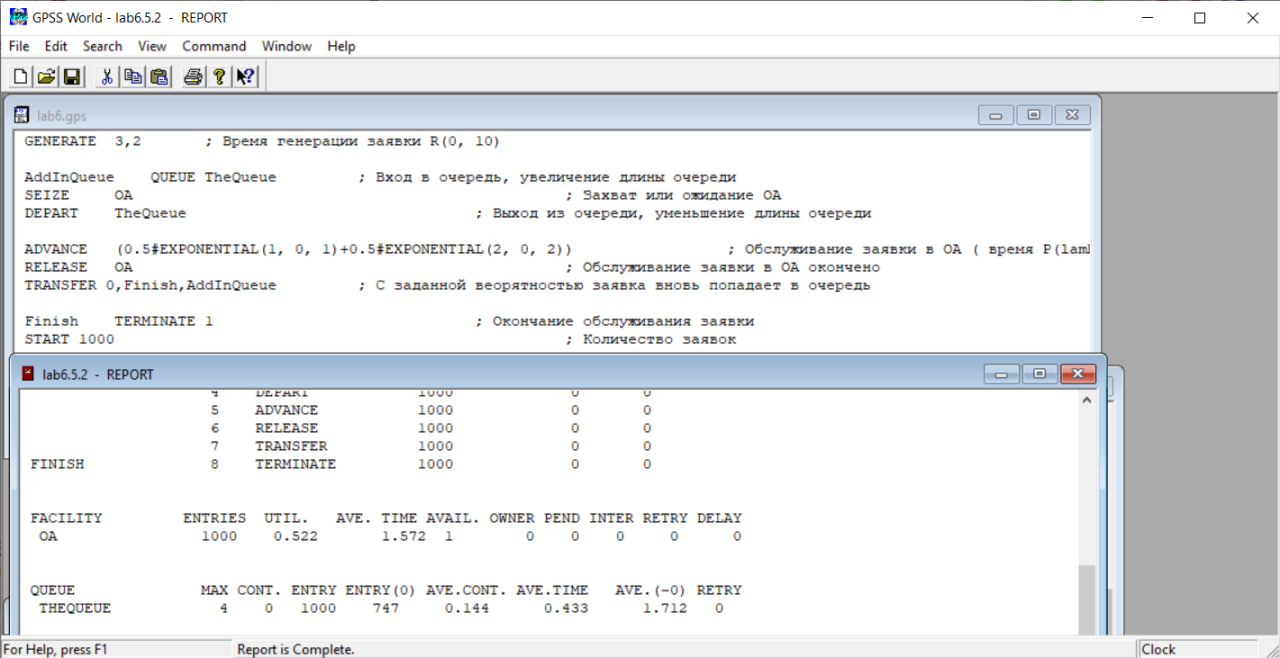
\includegraphics[scale=0.47]{pictures/demo.jpg}
			\caption{Результаты исследования программы}
			\label{pic:1}}
	\end{center}
\end{figure}

\end{document}